\section{Introduction du sujet}
	\subsection{Eternity II}
	
	\begin{frame}{Histoire}
		\begin{columns}
			\begin{column}{0.49\linewidth}
				\begin{figure}[H]
					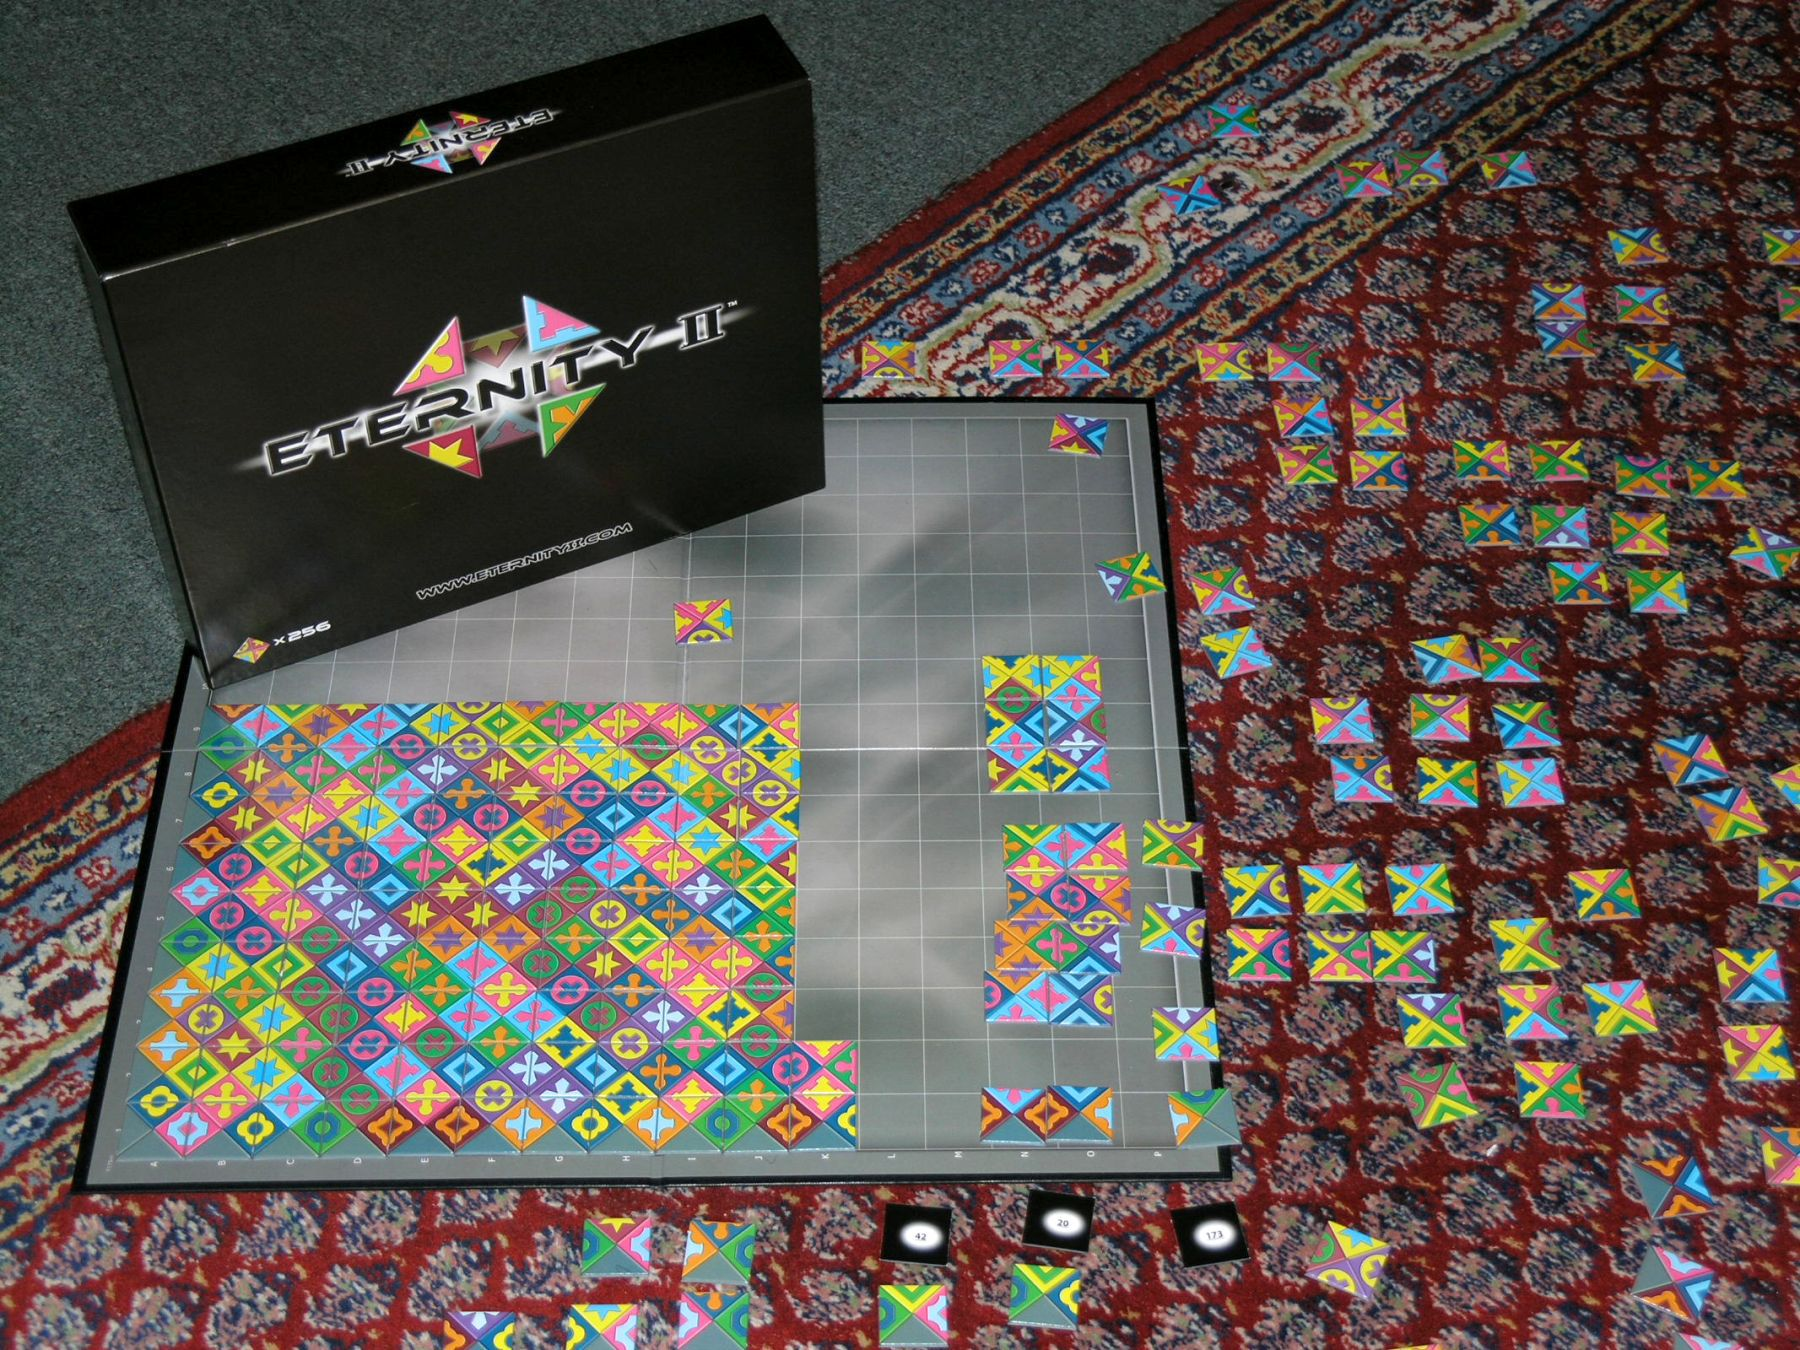
\includegraphics[width=\linewidth]{images/eternity_2}
				\end{figure}
			\end{column}
			\begin{column}{0.49\linewidth}
				\begin{Vblock}{Eternity II}
					\begin{itemize}[<+->]
						\item Succède à Eternity
						\item Sorti en 2008, avec à la clé \textdollar$2000000$
						\item Créés par Christopher Monckton
					\end{itemize}
				\end{Vblock}
			\end{column}
		\end{columns}
	\end{frame}

	\begin{frame}{Fonctionnement}
		%position absolue
		\begin{tikz}[remember picture, overlay]
			\node[anchor=north east] at (current page.north east) {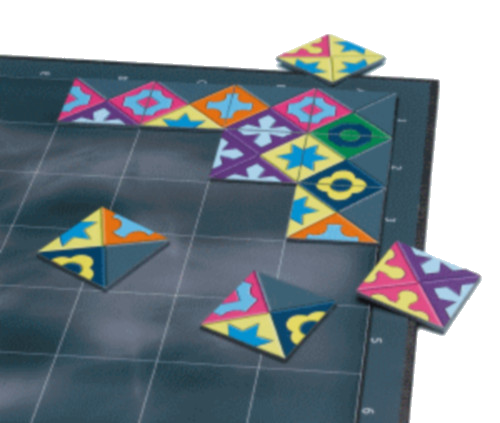
\includegraphics[width=0.25\linewidth]{images/puzzle_coin}};
		\end{tikz}
		C'est un puzzle composé d'un plateau de 16x16 et de 256 pièces carrées.
		
		\begin{Vblock}{3 types de pièces}
			\begin{minipage}{0.32\textwidth}
				\begin{figure}[H]
					\textbf{PC} : pièces de coin
					
\includegraphics[width=\textwidth]{images/piece_coin}
				\end{figure}
			\end{minipage}\hfill
			\pause
			\begin{minipage}{0.32\textwidth}
				\begin{figure}[H]
					\textbf{PB} : pièces de bord
					
\includegraphics[width=\textwidth]{images/piece_bord}
				\end{figure}
			\end{minipage}\hfill
			\pause
			\begin{minipage}{0.32\textwidth}
				\begin{figure}[H]
					\textbf{PI} : pièces d'intérieur
					
\includegraphics[width=\textwidth]{images/piece_interieure}
				\end{figure}
			\end{minipage}
		\end{Vblock}
	\end{frame}
	
	\begin{frame}{Fonctionnement}
		\begin{Bblock}{Matching}
			\begin{figure}
				
\includegraphics[width=0.5\linewidth]{images/matching_pieces}
			\end{figure}
		\end{Bblock}
	\end{frame}

	\subsection{Problématique}
	
	\begin{frame}{Problème actuel}
		\begin{itemize}[<+->]
			\item Non résolu depuis 8 ans
			\item Problème NP-complet (très complexe).
			\item Trop de possibilités (estimés à $10^{545}$).
			\item plateau de plus petite taille ($10\times 10$ non résolu).
		\end{itemize}
		\uncover<+->{
			\begin{Bblock}{Hypothèse}
				En s'axant sur une approche combinatoire.
				
				Réduire l'espace à énumérer en pré-calculant des surfaces du plateau. 
			\end{Bblock}}
	\end{frame}